\documentclass[tikz]{standalone}
\usepackage{pgfplots}
\usepackage{xcolor}
\usetikzlibrary{calc}
\definecolor{mycolor}{HTML}{ffd966}
\pgfplotsset{compat=1.18}

\begin{document}
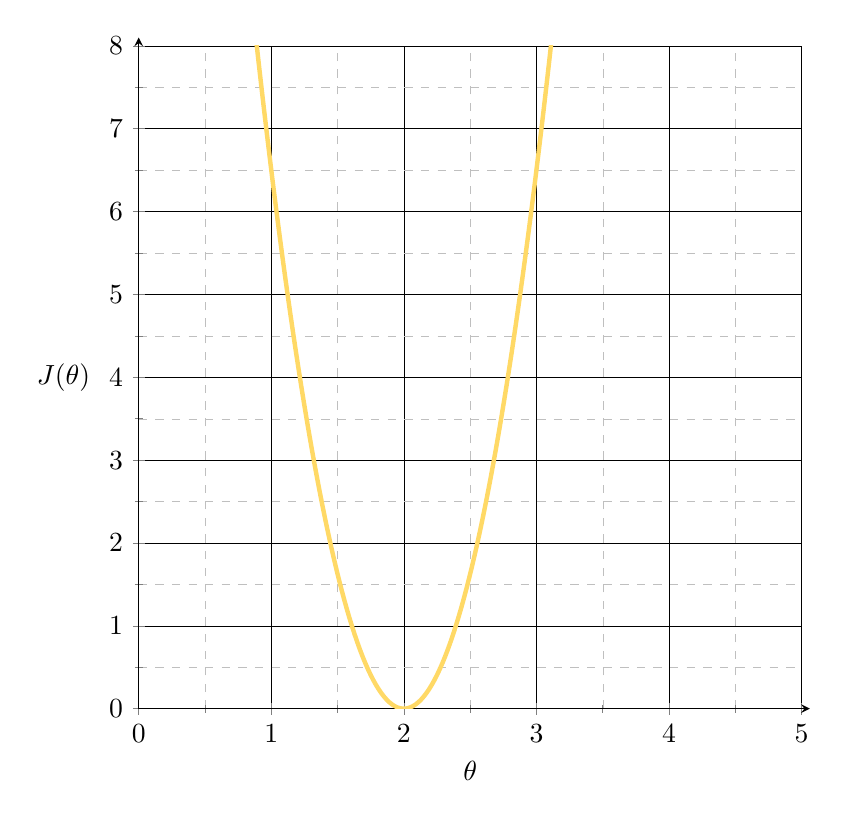
\begin{tikzpicture}
  \begin{axis}[
    axis lines=left,
    x axis line style={->,>=stealth, shorten >=-3pt},
    y axis line style={->,>=stealth, shorten >=-3pt},
    xlabel={\(\theta\)},
    ylabel={\(J(\theta)\)},
    ylabel style={rotate=-90},
    xmin=0, xmax=5,
    ymin=0, ymax=8,
    xtick={0,1,...,5},
    ytick={0,1,...,8},
    minor x tick num=1,
    minor y tick num=1,
    grid=both,
    major grid style={line width=0.2pt,draw=black},
    minor grid style={line width=0.1pt,draw=gray!50,dashed},
    width=10cm,
    height=10cm,
  ]
    % J(theta) = (1/2) * [(2*theta - 4)^2 + (3*theta - 6)^2]
    % Expanded: J(theta) = (1/2) * [13*theta^2 - 52*theta + 52]
    % Minimum at theta* = 52/(2*13) = 2
    \addplot[domain=0:4, samples=200, ultra thick, color=mycolor]
      {(1/2) * (13*x^2 - 52*x + 52)};
  \end{axis}
\end{tikzpicture}
\end{document}
